%!TEX root = ../rapport.tex

\chapter{Properties of $\beta$-reduction Graphs}

The preceding discussion of graph drawing concerns the problem of drawing
\emph{general} graphs. However, we focus not on general but on one specific
kind of graph: the $\beta$-reduction graph. It is important to identify the
most important characteristics of this graph type in order to be able to
choose relevant and meaningful drawing methods. Also, identifying the
properties that we actually want to highlight is relevant both for the
implementation of the functions that generate the reduction graphs as well as
for the functions that issue the actual drawing commands.

\section{Size}

Reduction graphs vary greatly in size, from one node to an infinite amount of
nodes and edges. For example, $G_\beta(\lam{x}{x})$ contains one node and zero
edges since there are no reducts in the term. On the other hand, the graph
$G_\beta((\lam{x}{xxx})(\lam{x}{xxx}))$ contains infinitely many nodes and
edges. 

In Figure \ref{fig:images_inf_reduction_graph} there are two different
drawings of (a part of) the graph $G_\beta((\lam{a}{b}) (\lam{x}{(xxx)}
\lam{y}{(yyy)}))$. This graph has infinitely many edges and nodes, so the
structure seen in the Figure will continue to grow. 

The layout algorithms are presented in Chapter \ref{chap:implementation}.

\fact
$\beta$-reduction graphs can have an infinite amount of nodes and edges.
\begin{figure}[htpb]
	% #a.(b) (#x.((x x) x) #y.((y y) y))
	\centering
	\subfigure[Drawn using the Circo algorithm.]{
		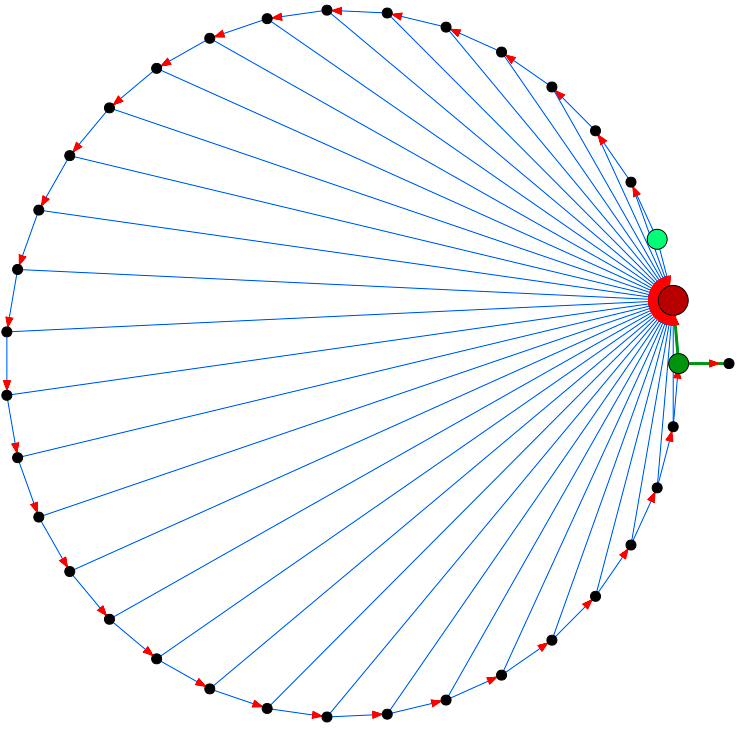
\includegraphics[height=2.2in]{../images/inf_reduction_graph_CIRCO.png}
	}
	\subfigure[Drawn using the Fdp algorithm.]{
		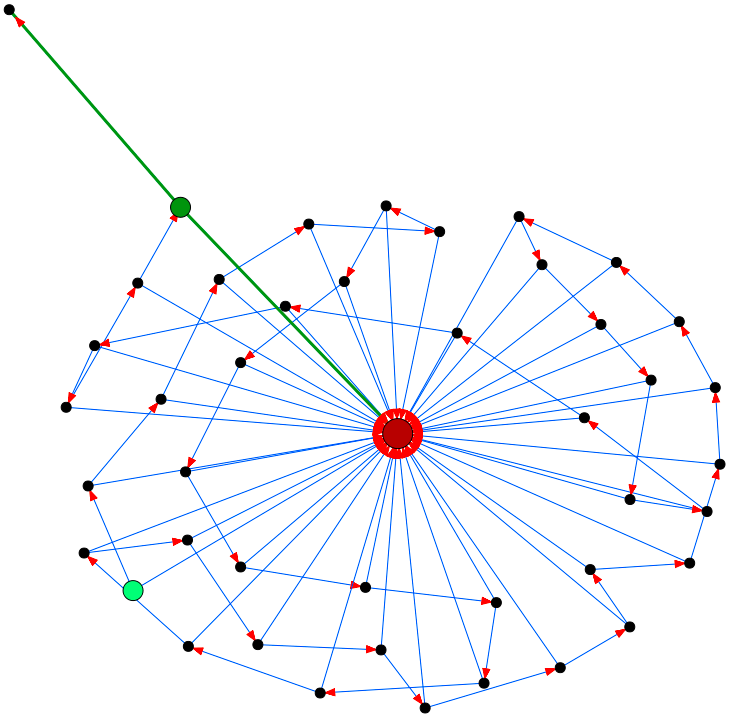
\includegraphics[height=2.2in]{../images/inf_reduction_graph_FDP.png}
	}
	\caption
	[$(\lam{a}{b}) (\lam{x}{(xxx)} \lam{y}{(yyy)})$]
	{$G_\beta\big((\lam{a}{b}) (\lam{x}{(xxx)} \lam{y}{(yyy)})\big)$. The normal form is drawn
	as a larger node. This is one generation of the reduction graph, but it 
	continues ad infinitum.}
	\label{fig:images_inf_reduction_graph}
\end{figure}


% Flere eksempler?

\section{Non-planarity}

As a consequence of Lemma \ref{lem:complete} we know that in the general case,
a reduction graph can contain as its subgraph $K_5$, whence the graph is
non-planar according to Kuratowski's theorem. Thus, it is in general not
possible to planarize a reduction graph. In Figure \ref{fig:images_lambda_k5}
a reduction graph whose underlying undirected graph \emph{is} $K_5$ is shown.

\begin{lemma}\label{lem:complete}
	$\forall n\in\N:\ \exists M\in\Lambda$ such that the $\beta$-reduction graph of $M$
	contains the complete (undirected) graph of $n$ nodes, $K_n$.
\end{lemma}
\begin{proof}[Proof (after a sketch by Jakob Grue Simonsen)]
	Let $n\in\N$, and let $M\in\Lambda$ be
	\begin{equation*}
		(\lam{x_1}{y}) ((\lam{x_2}{y}) ((\lam{x_3}{y})\hdots(\lam{x_{n}}{y})))
	\end{equation*}
	where $x_1\hdots x_n$ are distinct variable names. $M$ has $n-1$ distinct reducts of the form
	\begin{align*}
		&(\lam{x_1}{y}), \\
		&(\lam{x_1}{y})((\lam{x_2}{y}) y), \\
		&(\lam{x_1}{y})((\lam{x_2}{y}) ((\lam{x_3}{y}) y)),\ \hdots
	\end{align*}
	Call them $r_1,\hdots,r_{n-1}$ from least to greatest. For every
	$1\leq i < j \leq n-1$ we have $r_j\barrow r_i$. Thus, since $M\barrow r_i$ 
	for $1\leq i \leq n-1$, we have for every pair $(N_0,N_1)$ in the $\beta$-reduction 
	graph that $N_0\barrow N_1$ or $N_1\barrow N_0$, whence the underlying 
	undirected graph of the reduction graph is $K_n$.
\end{proof}

\begin{figure}[htpb]
	% (#x1.(y)) ((#x2.(y)) ((#x3.(y)) ((#x4.(y)) (#x5.(y)))))
	\centering
	\subfigure[Drawn using the Neato algorithm.]{
		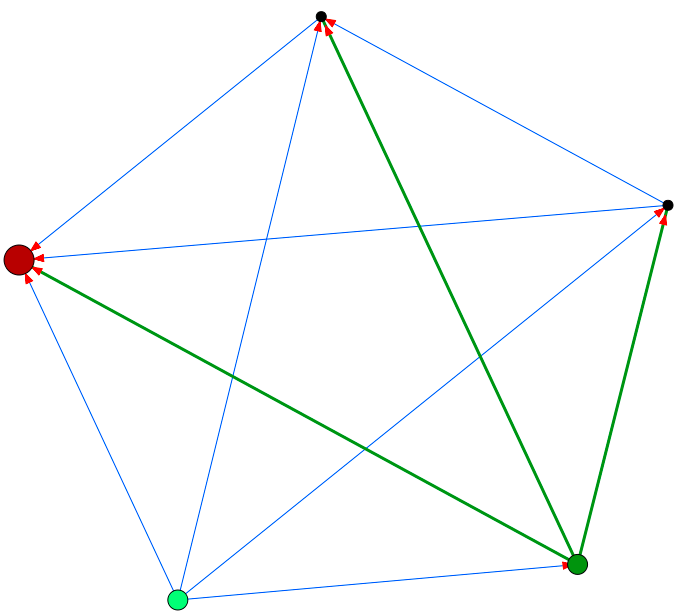
\includegraphics[height=2.2in]{../images/lambda_k5_NEATO.png}
	}
	\subfigure[Drawn using the Dot algorithm.]{
		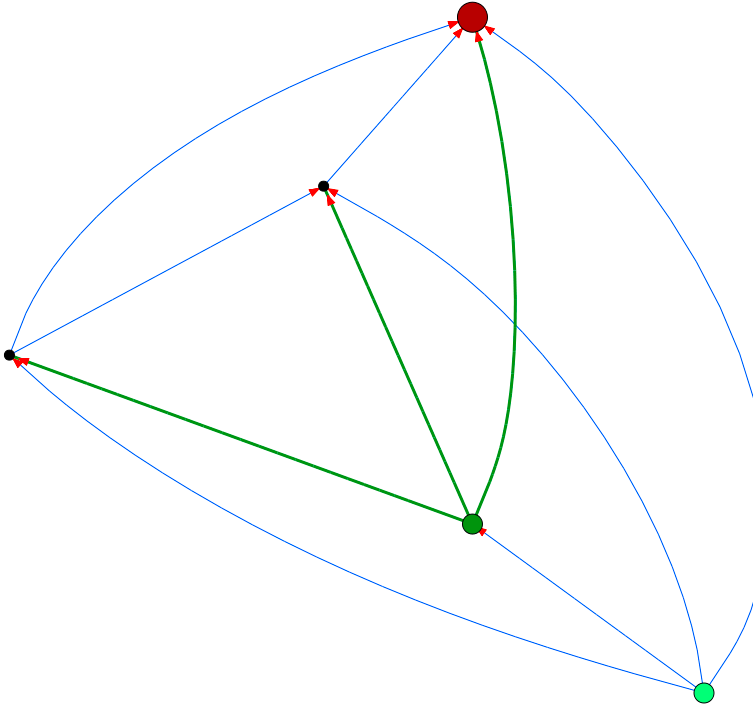
\includegraphics[height=2.2in]{../images/lambda_k5_DOT.png}
	}
	\caption
	[$(\lam{x_1}{y}) ((\lam{x_2}{y}) ((\lam{x_3}{y}) ((\lam{x_4}{y}) (\lam{x_5}{y})))$]
	{$G_\beta\big((\lam{x_1}{y}) ((\lam{x_2}{y}) ((\lam{x_3}{y}) ((\lam{x_4}{y}) (\lam{x_5}{y}))))\big)$
	from the proof of Lemma \ref{lem:complete}.}
	\label{fig:images_lambda_k5}
\end{figure}

\section{In- and out-degree of nodes}

The in- and out-degree of nodes varies a lot; the amount of redexes can be
very different from term to term, resulting in varying out-degrees, while some
nodes can have a potientially infinitely high in-degree.

For example, in the reduction graph for the term $(\lam{a}{b}) (\lam{x}{(xxx)}
\lam{y}{(yyy)})$, every node has an out-degree equal to 2 and an in-degree of
1, except the nodes representing the normal form and the initial term. The
former has an infinitely high in-degree and an out-degree of 0, the latter has
an in-degree of 0. The graph is illustrated on Figure \ref{fig:images_inf_reduction_graph}.

Since a particular lambda term in a reduction graph is finite, it necessarily has
a finite amount of redexes. The out-degree of the nodes representing the terms
is therefore finite.

% #a.(b) (#x.((x x) x) #y.((y y) y)) #a.(b) (#x.((x x) x) #y.((y y) y))
% #a.(b) ((#x.((x x) x) #y.((y y) y)) (#x.((x x) x) #y.((y y) y)))
% #a.(b) ((#a.(b) (#x.((x x) x) #y.((y y) y))) (#x.((x x) x) #y.((y y) y)))
% (#x1.(y)) ((#x2.(y)) ((#x3.(y)) ((#x4.(y)) (#x5.(y)))))

% Den her ser ret sej ud omkring nr. 100!
% #f.(#x.(f (x x))) (#x.(f (x x))) #y.((y y) y)

\fact Nodes can have an infinitely high in-degree.

\fact Nodes have a finite out-degree.

\fact The node representing the initial term can have an in-degree of 0.

\fact Since there always exists a path from the start node to all other nodes
in the reduction graph, the underlying undirected graph of a $\beta$-reduction
graph is connected. Hence, if there exists a node with an in-degree of 0, it
is the initial node.

\begin{figure}[tpb]
	% (#x.((x x) x) #y.((y y) y))
	\centering
	\subfigure[Drawn with the Neato algorithm.]{
		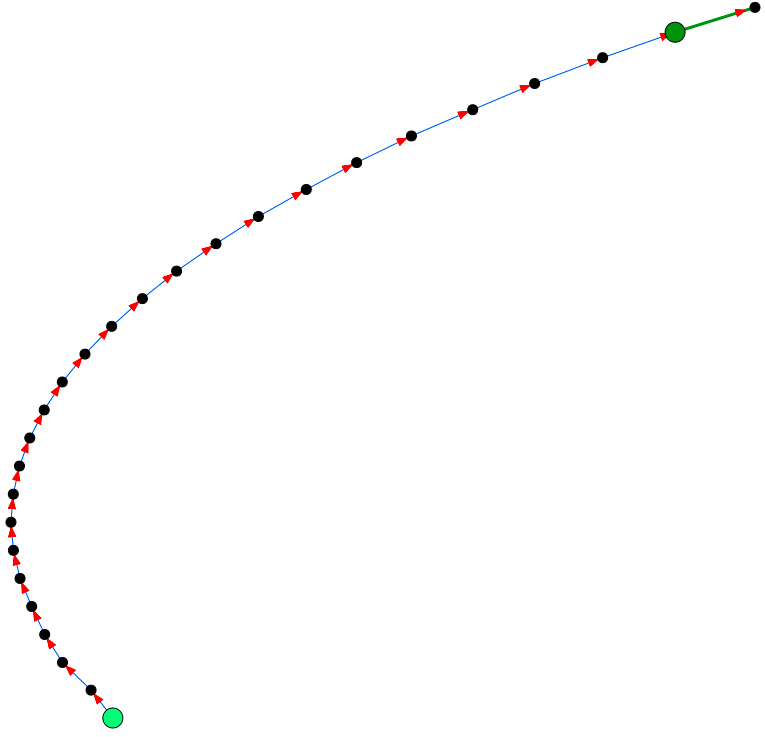
\includegraphics[height=2.2in]{../images/inf_reduction_graph_2_NEATO.png}
	}
	\subfigure[Drawn with the Fdp algorithm.]{
		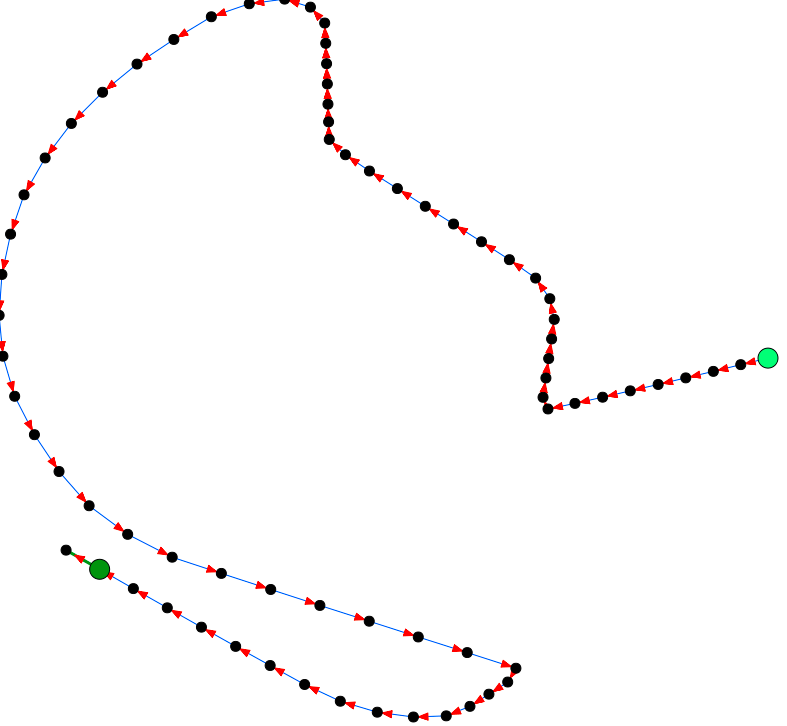
\includegraphics[height=2.2in]{../images/inf_reduction_graph_2_FDP.png}
	}
	\caption
	[$\lam{x}{(xxx)} \lam{y}{(yyy)}$]
	{$G_\beta\big(\lam{x}{(xxx)} \lam{y}{(yyy)}\big)$}
	\label{fig:images_inf_reduction_graph_2}
\end{figure}

\section{Normal Forms}

If the term whose reduction graph is visualized has a normal form, it is
desirable to be able to easily see it, even when there are a lot of nodes in
the graph. Therefore, a clear graphical hint must be added to the node that
represent a normal form. This could for instance be implemented as giving the
normal form node a certain colouring, a certain size or draw it with a
different shape than the other nodes (e.g. square vs. circular).

\fact Regardless of whether a term has a normal form or not, the amount
of edges and nodes in its reduction graph can be infinite; see for instance Figure 
\ref{fig:images_inf_reduction_graph_2} and \ref{fig:images_inf_reduction_graph}.
Similarly, both terms with and without normal forms can have finite reduction graphs;
see e.g. Figure \ref{fig:images_lambda_k5} and \ref{fig:images_Circle_1}.

% \fact Terms without normal forms have reduction graphs with infinitely many
% nodes and edges (e.g. the graph in Figure \ref{fig:images_inf_reduction_graph_2}). 
% 
% \fact Terms with normal forms have possibly infinite reduction graphs (e.g.
% the graph in Figure \ref{fig:images_inf_reduction_graph}).
